\begin{figure*}
	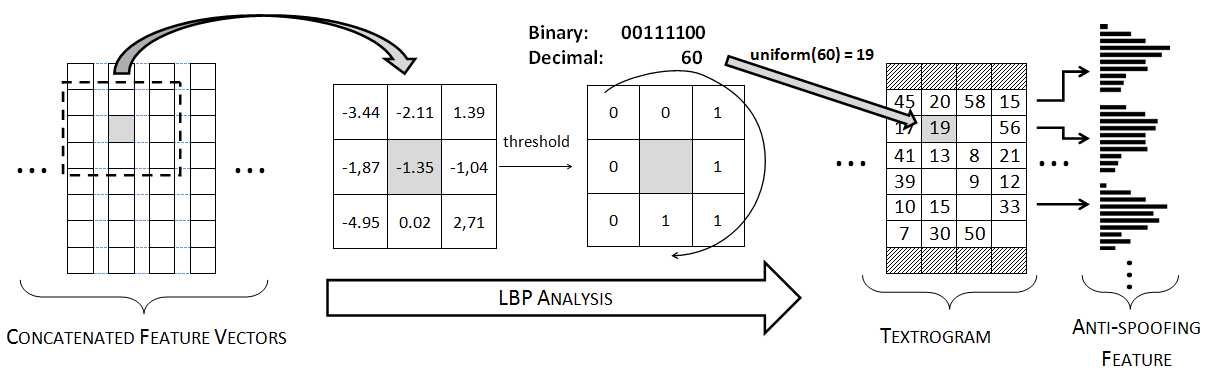
\includegraphics[width=1\linewidth]{Figs/LBP_idea.png}
	\caption{Schematic diagram of LBP-based feature extraction.}
%{\bfseries Can you hyphenate antispoofing?  I also suggest to reduce the size of the speech utterance and feature extraction arrow in order that you can increase the size of the textrogram, histograms and fontsizes.  Possibly, remove the speech utterance and feature extraction arros entirely.}
	\label{fig:LBPfeature}
\end{figure*}

Attention now turns to the detection of replay spoofing attacks with dedicated countermeasures.  Given that only little work has investigated ASV vulnerabilities to such attacks, it is hardly surprising that work to develop countermeasures is similarly limited.  This section briefly reviews that past work and then describes two particular replay countermeasures which are explored further in this paper.



\subsection{General approaches}

One obvious approach to replay detection involves challenge-response systems which require the speaker to utter a prompted phrase~\cite{Petrovska1998}. 
Challenge-response mechanisms are a form of passive countermeasure.
While having potential in preventing some forms of replay attack for some ASV systems, challenge-response countermeasures are not without impacts on usability which may render them undesirable for other ASV systems.  Challenge-response systems also lack sufficient scientific validation.

Active countermeasures have also been proposed.  One such approach, based upon the detection of so-called pop noise, is proposed in~\cite{Shiota2015}.  Pop noise is a short-duration, typically low-frequency artefact resulting from the impact of natural speech upon a close-talk microphone.  Since most loudspeakers exhibit poor fidelity at low frequencies, pop noise is normally attenuated upon replay.  The absence of natural pop noise thus serves as an indicator of replay attacks.  Two different approaches to measure pop noise are described in~\cite{Shiota2015}.  The first, single-channel method is based upon estimates of low-frequency energy, which is characteristic of pop noise.  The second, double-channel method, is based upon the difference between two signals captured by two microphones, one of which is equipped with a pop noise filter.  Results show that replay attacks can be detected with an EER of as little as 4\% where speech is captured using a headset microphone.  Performance is, however, greatly reduced in the case of telephony speech; pop noise is in any case attenuated as a result of narrowband transmission.

A different approach involves the storing of previous access attempts and their comparison to new attempts~\cite{Shang2010}.
New access attempts which are deemed too close to previous attempts are rejected.
A somewhat similar technique is proposed in~\cite{Wu2014}, where the authors compare spectral bitmaps between access trials and previously stored recordings in a text-dependent ASV scenario. 

A alternative method of detecting replay attacks was proposed recently in~\cite{Galka2015}.  It is based on the distances between landmark points in the amplitude spectrum of the speech signal.  When assessed in a fixed-phrase scenario with data collected from 175 speakers, a detection EER of 1\% was achieved.  The detection of high similarity thus serves as an effective means of identifying replay attacks, albeit in somewhat constrained scenarios.

Other, more generally applicable methods, not restricted to a specific ASV scenario, are based on the detection of unexpected channel artefacts indicative of recording and replaying.
Two such algorithms are reported in~\cite{Wang2011} for which the EER for a baseline Gaussian mixture model (GMM) system with a universal background model (UBM) was shown to decrease from 40\% to 10\% with active countermeasures.  

A more recent study~\cite{Luo2015} describes the application of a deep neural network to detect replayed speech.  
%The authors trained such a network to extract necessary information directly from speech samples. 
When assessed on the standard Wall Street Journal (WSJ) corpus~\cite{WSJ1993}, adapted to the assessment of replay attack spoofing, a detection EER of 7.5\% was achieved.  The detection of channel artefacts is also the basis of the first approach investigated further in this paper.




\subsection{Far-field channel detection}
\label{subsec:ffd}

Many scenarios in which user authentication is performed by ASV involve so-called close-talk speech, i.e.\ situations where speech is collected from an in situ or closely positioned microphone.  Examples include telephony and logical access scenarios or critical infrastructure protection and physical access scenarios.  In contrast, since they are likely to be collected surreptitiously or at-distance, replay recordings may exhibit far-field channel effects, effects which can be measured and consequently used to detect replayed speech.  

This idea was first investigated in~\cite{Villalba2011}.  The work compares close-talk and far-field speech signals parametrised according to 12 channel-sensitive features:


\begin{itemize}
\item spectral ratio -- sub-band energy ratio from 0-2~kHz and from 2-4~kHz; 
\item low frequency ratio -- sub-band energy ratio from 100-300~Hz and from 300-500~Hz, calculated using speech frames only;
\item modulation index, and
\item nine sub-band modulation indices -- see~\cite{Villalba2011} for precise sub-band bandwidths.
\end{itemize}


The spectral ratio reflects the level of spectrum flattening or noise and reverberation introduced by far-field recording.  The low frequency ratio reflects the (potentially heightened) level of high-pass filtering, an artefact typical of speech signals produced by small loudspeakers.  The total and sub-band modulation indices reflect the level of additive and, specifically, coloured noise; higher levels of noise present in replay recordings result in lower than average modulation indices.  Experiments were performed with a support vector machine (SVM) classifier and showed that far-field recordings could be detected with 90\% accuracy.  %%{\bfseries what classifier?}



\subsection{Local binary patterns}


The approach to replay detection proposed in~\cite{Alegre2014} is based on the local binary pattern (LBP) analysis of speech spectrograms.  
Inspired by the original application to image texture analysis~\cite{Ojala2002}, the idea was introduced as an ASV spoofing countermeasure in~\cite{Alegre2013a}.  
As illustrated in Fig.~\ref{fig:LBPfeature}, LBP analysis is applied to a Mel-scaled cepstrogram with appended dynamic features.  Modifications made through spoofing are assumed to disturb the natural `texture' of genuine speech, attributes which are readily detected with LBP.   

The standard LBP operator is a non-parametric 3x3 kernel which assigns a binary code to each pixel in an image according to the comparison of its intensity value to that of its eight surrounding pixels~\cite{Ojala2002}. 
A binary value of 1 is assigned when the intensity of neighbouring pixels (here feature components) is higher, whereas a value of 0 is assigned when neighbouring pixels are of lower or equal intensity. Each pixel is thus assigned one of $2^8=256$ binary patterns. As is common in other applications, e.g. that in face recognition~\cite{Ahonen2006}, only a subset of the so-called uniform binary patterns are used, i.e.,  LBPs which contain at most two bitwise transitions from 0 to 1 or 1 to 0 when the bit pattern is traversed in circular fashion.

LBPs can be determined for each pixel in a Mel-scaled cepstrogram thus resulting in a new matrix of reduced dynamic range, here referred to as a \emph{textrogram}.  
The textrogram captures short-time feature motion beyond that in conventional dynamic parametrisations.  
Normalised histograms of pixel values constructed for each row of the textrogram   are stacked vertically to obtain the anti-spoofing feature vector in the same manner as GMM mean-vectors are stacked to form supervectors.  
In the work reported here, LBP-based features are calculated for the both the enrolment and test data.  The two resulting feature vectors are compared using histogram intersection and the resulting score is thresholded to decide if the test signal is genuine speech or a spoofing attack.
%{\bfseries What classifier - how are the anti-spoofing feature vectors used?}

Experimental results presented in~\cite{Alegre2013a} showed that the LBP-based textrogram analysis is effective in detecting a range of spoofed speech signals, including artificial signals, speech synthesis (EERs of below 1\%) and voice conversion (EER in the order of 7\%).  The motivation for using LBP analysis as a means of detecting replay attacks is described in Section~IV-D.
